%\documentclass[10pt,handout]{beamer}
\documentclass[10pt]{beamer}
\usepackage[english]{babel} % Anpassa efter svenska. Ger svensk logga.
\usepackage[utf8]{inputenc} % Anpassa efter linux
\usepackage{graphicx}
\usepackage{hyperref}
\usepackage{listings}
\lstdefinelanguage{Stan}{
  morekeywords=[1]{functions,data,parameters,transformed,model,generated,quantities,%
    for,in,while,print,if,else,lower,upper,increment_log_prob,T,return,%
    reject,integrate_ode,integrate_ode_bdf,integrate_ode_rk45,target},%
  morekeywords=[2]{int,real,vector,%
    ordered,positive_ordered,simplex,unit_vector,%
    row_vector,matrix,%
    cholesky_factor_corr,cholesky_factor_cov,%
    coor_matrix,cov_matrix,%
    void},%
  morekeywords=[3]{%
    Phi,%
    Phi_approx,%
    abs,%
    acos,%
    acosh,%
    append_col,%
    append_row,%
    asin,%
    asinh,%
    atan,%
    atan2,%
    atanh,%
    bernoulli_cdf,%
    bernoulli_cdf_log,%
    bernoulli_lccdf,%
    bernoulli_lcdf,%
    bernoulli_logit_lpmf,%
    bernoulli_logit_lpmf,%
    bernoulli_lpmf,%
    bernoulli_lpmf,%
    bernoulli_rng,%
    bessel_first_kind,%
    bessel_second_kind,%
    beta_binomial_cdf,%
    beta_binomial_cdf_log,%
    beta_binomial_lccdf,%
    beta_binomial_lcdf,%
    beta_binomial_lpmf,%
    beta_binomial_lpmf,%
    beta_binomial_rng,%
    beta_cdf,%
    beta_cdf_log,%
    beta_lccdf,%
    beta_lcdf,%
    beta_lpdf,%
    beta_lpdf,%
    beta_rng,%
    binary_log_loss,%
    binomial_cdf,%
    binomial_cdf_log,%
    binomial_coefficient_log,%
    binomial_lccdf,%
    binomial_lcdf,%
    binomial_logit_lpmf,%
    binomial_logit_lpmf,%
    binomial_lpmf,%
    binomial_lpmf,%
    binomial_rng,%
    block,%
    categorical_logit_lpmf,%
    categorical_logit_lpmf,%
    categorical_lpmf,%
    categorical_lpmf,%
    categorical_rng,%
    cauchy_cdf,%
    cauchy_cdf_log,%
    cauchy_lccdf,%
    cauchy_lcdf,%
    cauchy_lpdf,%
    cauchy_lpdf,%
    cauchy_rng,%
    cbrt,%
    ceil,%
    chi_square_cdf,%
    chi_square_cdf_log,%
    chi_square_lccdf,%
    chi_square_lcdf,%
    chi_square_lpdf,%
    chi_square_lpdf,%
    chi_square_rng,%
    cholesky_decompose,%
    col,%
    cols,%
    columns_dot_product,%
    columns_dot_self,%
    cos,%
    cosh,%
    crossprod,%
    csr_extract_u,%
    csr_extract_v,%
    csr_extract_w,%
    csr_matrix_times_vector,%
    csr_to_dense_matrix,%
    cumulative_sum,%
    determinant,%
    diag_matrix,%
    diag_post_multiply,%
    diag_pre_multiply,%
    diagonal,%
    digamma,%
    dims,%
    dirichlet_lpdf,%
    dirichlet_lpdf,%
    dirichlet_rng,%
    distance,%
    dot_product,%
    dot_self,%
    double_exponential_cdf,%
    double_exponential_cdf_log,%
    double_exponential_lccdf,%
    double_exponential_lcdf,%
    double_exponential_lpdf,%
    double_exponential_lpdf,%
    double_exponential_rng,%
    e,%
    eigenvalues_sym,%
    eigenvectors_sym,%
    erf,%
    erfc,%
    exp,%
    exp2,%
    exp_mod_normal_cdf,%
    exp_mod_normal_cdf_log,%
    exp_mod_normal_lccdf,%
    exp_mod_normal_lcdf,%
    exp_mod_normal_lpdf,%
    exp_mod_normal_lpdf,%
    exp_mod_normal_rng,%
    expm1,%
    exponential_cdf,%
    exponential_cdf_log,%
    exponential_lccdf,%
    exponential_lcdf,%
    exponential_lpdf,%
    exponential_lpdf,%
    exponential_rng,%
    fabs,%
    falling_factorial,%
    fdim,%
    floor,%
    fma,%
    fmax,%
    fmin,%
    fmod,%
    frechet_cdf,%
    frechet_cdf_log,%
    frechet_lccdf,%
    frechet_lcdf,%
    frechet_lpdf,%
    frechet_lpdf,%
    frechet_rng,%
    gamma_cdf,%
    gamma_cdf_log,%
    gamma_lccdf,%
    gamma_lcdf,%
    gamma_lpdf,%
    gamma_lpdf,%
    gamma_p,%
    gamma_q,%
    gamma_rng,%
    gaussian_dlm_obs_lpdf,%
    gaussian_dlm_obs_lpdf,%
    get_lp,%
    gumbel_cdf,%
    gumbel_cdf_log,%
    gumbel_lccdf,%
    gumbel_lcdf,%
    gumbel_lpdf,%
    gumbel_lpdf,%
    gumbel_rng,%
    head,%
    hypergeometric_lpmf,%
    hypergeometric_lpmf,%
    hypergeometric_rng,%
    hypot,%
    if_else,%
    inc_beta,%
    int_step,%
    inv,%
    inv_chi_square_cdf,%
    inv_chi_square_cdf_log,%
    inv_chi_square_lccdf,%
    inv_chi_square_lcdf,%
    inv_chi_square_lpdf,%
    inv_chi_square_lpdf,%
    inv_chi_square_rng,%
    inv_cloglog,%
    inv_gamma_cdf,%
    inv_gamma_cdf_log,%
    inv_gamma_lccdf,%
    inv_gamma_lcdf,%
    inv_gamma_lpdf,%
    inv_gamma_lpdf,%
    inv_gamma_rng,%
    inv_logit,%
    inv_phi,%
    inv_sqrt,%
    inv_square,%
    inv_wishart_lpdf,%
    inv_wishart_lpdf,%
    inv_wishart_rng,%
    inverse,%
    inverse_spd,%
    is_inf,%
    is_nan,%
    lbeta,%
    lchoose,%
    lgamma,%
    lkj_corr_cholesky_lpdf,%
    lkj_corr_cholesky_lpdf,%
    lkj_corr_cholesky_rng,%
    lkj_corr_lpdf,%
    lkj_corr_lpdf,%
    lkj_corr_rng,%
    lmgamma,%
    lmultiply,%
    log,%
    log10,%
    log1m,%
    log1m_exp,%
    log1m_inv_logit,%
    log1p,%
    log1p_exp,%
    log2,%
    log_determinant,%
    log_diff_exp,%
    log_falling_factorial,%
    log_inv_logit,%
    log_mix,%
    log_rising_factorial,%
    log_softmax,%
    log_sum_exp,%
    logistic_cdf,%
    logistic_cdf_log,%
    logistic_lccdf,%
    logistic_lcdf,%
    logistic_lpdf,%
    logistic_lpdf,%
    logistic_rng,%
    logit,%
    lognormal_cdf,%
    lognormal_cdf_log,%
    lognormal_lccdf,%
    lognormal_lcdf,%
    lognormal_lpdf,%
    lognormal_lpdf,%
    lognormal_rng,%
    machine_precision,%
    max,%
    mdivide_left_tri_low,%
    mdivide_right_tri_low,%
    mean,%
    min,%
    modified_bessel_first_kind,%
    modified_bessel_second_kind,%
    multi_gp_cholesky_lpdf,%
    multi_gp_cholesky_lpdf,%
    multi_gp_lpdf,%
    multi_gp_lpdf,%
    multi_normal_cholesky_lpdf,%
    multi_normal_cholesky_lpdf,%
    multi_normal_cholesky_rng,%
    multi_normal_lpdf,%
    multi_normal_lpdf,%
    multi_normal_prec_lpdf,%
    multi_normal_prec_lpdf,%
    multi_normal_rng,%
    multi_student_t_lpdf,%
    multi_student_t_lpdf,%
    multi_student_t_rng,%
    multinomial_lpmf,%
    multinomial_lpmf,%
    multinomial_rng,%
    multiply_log,%
    multiply_lower_tri_self_transpose,%
    neg_binomial_2_cdf,%
    neg_binomial_2_cdf_log,%
    neg_binomial_2_lccdf,%
    neg_binomial_2_lcdf,%
    neg_binomial_2_log_lpmf,%
    neg_binomial_2_log_lpmf,%
    neg_binomial_2_log_rng,%
    neg_binomial_2_lpmf,%
    neg_binomial_2_lpmf,%
    neg_binomial_2_rng,%
    neg_binomial_cdf,%
    neg_binomial_cdf_log,%
    neg_binomial_lccdf,%
    neg_binomial_lcdf,%
    neg_binomial_lpmf,%
    neg_binomial_lpmf,%
    neg_binomial_rng,%
    negative_infinity,%
    normal_cdf,%
    normal_cdf_log,%
    normal_lccdf,%
    normal_lcdf,%
    normal_lpdf,%
    normal_lpdf,%
    normal_rng,%
    not_a_number,%
    num_elements,%
    ordered_logistic_lpmf,%
    ordered_logistic_lpmf,%
    ordered_logistic_rng,%
    owens_t,%
    pareto_cdf,%
    pareto_cdf_log,%
    pareto_lccdf,%
    pareto_lcdf,%
    pareto_lpdf,%
    pareto_lpdf,%
    pareto_rng,%
    pareto_type_2_cdf,%
    pareto_type_2_cdf_log,%
    pareto_type_2_lccdf,%
    pareto_type_2_lcdf,%
    pareto_type_2_lpdf,%
    pareto_type_2_lpdf,%
    pareto_type_2_rng,%
    pi,%
    poisson_cdf,%
    poisson_cdf_log,%
    poisson_lccdf,%
    poisson_lcdf,%
    poisson_log_lpmf,%
    poisson_log_lpmf,%
    poisson_log_rng,%
    poisson_lpmf,%
    poisson_lpmf,%
    poisson_rng,%
    positive_infinity,%
    pow,%
    prod,%
    qr_Q,%
    qr_R,%
    quad_form,%
    quad_form_diag,%
    quad_form_sym,%
    rank,%
    rayleigh_cdf,%
    rayleigh_cdf_log,%
    rayleigh_lccdf,%
    rayleigh_lcdf,%
    rayleigh_lpdf,%
    rayleigh_lpdf,%
    rayleigh_rng,%
    rep_array,%
    rep_matrix,%
    rep_row_vector,%
    rep_vector,%
    rising_factorial,%
    round,%
    row,%
    rows,%
    rows_dot_product,%
    rows_dot_self,%
    scaled_inv_chi_square_cdf,%
    scaled_inv_chi_square_cdf_log,%
    scaled_inv_chi_square_lccdf,%
    scaled_inv_chi_square_lcdf,%
    scaled_inv_chi_square_lpdf,%
    scaled_inv_chi_square_lpdf,%
    scaled_inv_chi_square_rng,%
    sd,%
    segment,%
    sin,%
    singular_values,%
    sinh,%
    size,%
    skew_normal_cdf,%
    skew_normal_cdf_log,%
    skew_normal_lccdf,%
    skew_normal_lcdf,%
    skew_normal_lpdf,%
    skew_normal_lpdf,%
    skew_normal_rng,%
    softmax,%
    sort_asc,%
    sort_desc,%
    sort_indices_asc,%
    sort_indices_desc,%
    sqrt,%
    sqrt2,%
    square,%
    squared_distance,%
    step,%
    student_t_cdf,%
    student_t_cdf_log,%
    student_t_lccdf,%
    student_t_lcdf,%
    student_t_lpdf,%
    student_t_lpdf,%
    student_t_rng,%
    sub_col,%
    sub_row,%
    sum,%
    tail,%
    tan,%
    tanh,%
    tcrossprod,%
    tgamma,%
    to_array_1d,%
    to_array_2d,%
    to_matrix,%
    to_row_vector,%
    to_vector,%
    trace,%
    trace_gen_quad_form,%
    trace_quad_form,%
    trigamma,%
    trunc,%
    uniform_cdf,%
    uniform_cdf_log,%
    uniform_lccdf,%
    uniform_lcdf,%
    uniform_lpdf,%
    uniform_lpdf,%
    uniform_rng,%
    variance,%
    von_mises_lpdf,%
    von_mises_lpdf,%
    von_mises_rng,%
    weibull_cdf,%
    weibull_cdf_log,%
    weibull_lccdf,%
    weibull_lcdf,%
    weibull_lpdf,%
    weibull_lpdf,%
    weibull_rng,%
    wiener_lpdf,%
    wiener_lpdf,%
    wishart_lpdf,%
    wishart_lpdf,%
    wishart_rng
  },%
  otherkeywords={<-,~,+=,=},%
  sensitive=true,%
  morecomment=[l]{\#},%
  morecomment=[l]{//},%
  morecomment=[n]{/*}{*/},%
  string=[d]"%,
  literate={<-}{{$\leftarrow$}}1 {~}{{$\sim$}}1%
}
 % Stan listing[language=Stan]

\hypersetup{
    colorlinks=true,
    linkcolor=blue,
    filecolor=magenta,
    urlcolor=cyan,
}
\usepackage{../common/beamerthemeUppsala}
%\usetheme{Uppsala}
%\usecolortheme{UU} % Anpassa efter UU:s frger och logga
%\hypersetup{pdfpagemode=FullScreen} % Adobe Reader ska ppna fullskrm
\setbeamertemplate{itemize items}[circle]

% \usepackage{beamerthemesplit}
\usepackage{amsmath}
% \usepackage{amssymb}
% \usepackage{graphics}
% \usepackage{graphicx}
% \usepackage{epsfig}
% \usepackage[latin1]{inputenc}
 \usepackage{color}
% \usepackage{fancybox}
% \usepackage{psfrag}
% \usepackage[english]{babel}
 \setbeamertemplate{footline}{\hfill\insertframenumber/\inserttotalframenumber}

% Input new commands
%\usepackage{bm}
%\usepackage{natbib}
\newcommand{\bfm}[1]   {\mbox{\boldmath{${#1}$}}}
\newcommand{\Prob}   {\mbox{\textnormal{P}}}
\def\eqd{\,{\buildrel d \over =}\,}

% Vector/Matrix definitions (in bold type)
\newcommand{\vect}[1]{\mathbf{#1}}
\newcommand{\vectb}[1]{\bm{#1}}

% Differential operator 'd' as upright as in (use \dd)
\newcommand{\dd}{\; \mathrm{d}}

% Gaussian normal distribution (use \N)
\newcommand{\N}{\mathcal{N}} %% or \mathrm{N}

% Uniform distribution (use \Uni or \U)
\newcommand{\Uni}{\mathcal{U}} %% or \mathrm{U}
\newcommand{\U}{\mathcal{U}} %% or \mathrm{U}

% Matrix transpose (use \T)
\newcommand{\T}{^{\mathsf{T}}}

% Blockdiagonal matrices (use \blockdiag)
\newcommand{\blockdiag}{\mathrm{blockdiag}}

% Define inner product '<f,g>' notation (use \innerp{#1})
\providecommand{\innerp}[1]{\left\langle#1\right\rangle}

\def\o{{\mathbf o}}
\def\t{{\mathbf \theta}}
\def\w{{\mathbf w}}
\def\x{{\mathbf x}}
\def\y{{\mathbf y}}
\def\z{{\mathbf z}}



% Other math symbols and notation
\newcommand{\D}{^\mathsf{\dagger}}
\newcommand{\R}{\mathbb{R}}
\newcommand{\erf}{\mathrm{erf}}
\newcommand{\E}{\mathrm{E}}
\newcommand{\var}{\mathrm{var}}
\newcommand{\Var}{\mathrm{Var}}
\newcommand{\cov}{\mathrm{cov}}
\newcommand{\Ker}{\operatorname{Ker}}
\newcommand{\Ran}{\operatorname{Ran}}
\providecommand{\norm}[1]{\lVert#1\rVert}
\providecommand{\op}[1]{\mathcal{#1}}
\newcommand{\arccot}{\mathrm{arccot}}
\providecommand{\Hspace}[1]{\mathscr{#1}}
\providecommand{\fourier}[1]{\mathscr{#1}}

\newcommand{\kin}{k^{\rm in}}
\newcommand{\kout}{k^{\rm out}}
\newcommand{\gi}{{R_0}}
\newcommand{\eff}{{E_{\rm max}}}
\newcommand{\ESS}{\mathrm{ESS}}
\newcommand{\HN}{{\rm N^+}}
\newcommand{\lN}{{\rm LN}}

\DeclareMathOperator{\Sd}{Sd}
\DeclareMathOperator{\sd}{sd}
\DeclareMathOperator{\Gammad}{Gamma}
\DeclareMathOperator{\Invgamma}{Inv-gamma}
\DeclareMathOperator{\Bin}{Bin}
\DeclareMathOperator{\Negbin}{Neg-bin}
\DeclareMathOperator{\Poisson}{Poisson}
\DeclareMathOperator{\Beta}{Beta}
\DeclareMathOperator{\logit}{logit}
\DeclareMathOperator{\BF}{BF}
\DeclareMathOperator{\Invchi2}{Inv-\chi^2}
\DeclareMathOperator{\NInvchi2}{N-Inv-\chi^2}
\DeclareMathOperator{\InvWishart}{Inv-Wishart}
\DeclareMathOperator{\tr}{tr}
% \DeclareMathOperator{\Pr}{Pr}
\def\euro{{\footnotesize \EUR\, }}
\DeclareMathOperator{\rep}{\mathrm{rep}}


%%%%%%%%%%%%%%%%%%%%%%%%%%%%%%%%%%%%%%%%%%%%%%%%%%%%%%%%%%%%%%%%%%

\setlength{\parskip}{3mm}
\title[]{{\color{black}Bayesian Statistics and Data Analysis \\ Lecture 4}}
\author[]{M{\aa}ns Magnusson \\ Department of Statistics, Uppsala University \\ Thanks to Aki Vehtari, Aalto University}
\date{}

\begin{document}

\frame{\titlepage
% \thispagestyle{empty}
}

%%%%%%%%%%%%%%%%%%%%%%%%%%%%%%%%%%%%%%%%%%%%%%%%%%%%%%%%%%%%%%%%%%


% Be more clear in the evaluation. "Some questions could be more clear" I cant use that. Please state what can be more clear and why.



\begin{frame}

\frametitle{Assignment 3}

  \begin{itemize}
  \item Be more clear in the evaluation - where is the problem.
  \item Example: "Some questions could be more clear"% I cant use that. Please state what can be more clear and why.
  \end{itemize}

\end{frame}

\section{Introduction}
% \frame{\sectionpage}

\begin{frame}

\frametitle{Notation}

  \begin{itemize}
  \item In this chapter, generic $p(\theta)$ is used instead of
    $p(\theta|y)$
  \item Unnormalized distribution is denoted by $q(\cdot)$
    \begin{itemize}
    \item $\int q(\theta) d\theta \neq 1$, but finite (i.e. $\int q(\theta) d\theta \le \infty$
    \item $q(\cdot) \propto p(\cdot)$
    \end{itemize}
  \item Proposal distribution is denoted by $g(\cdot)$
  \end{itemize}

\end{frame}

\begin{frame}

\frametitle{Numerical accuracy -- floating point}

  \begin{itemize}
  \item Floating point presentation of numbers. e.g. with 64bits
    \begin{itemize}
    \item closest value to zero is $\approx 2.2\cdot 10^{-308}$
      \begin{itemize}
      \item generate sample of 600 from normal distribution:\\
        {\color{uured} qr=rnorm(600)}
      \item calculate joint density given normal:\\
        {\color{uured} prod(dnorm(qr)) $\rightarrow$} {\color{red} 0 (underflow)}
      \item<2-> see log densities in the next slide
      \end{itemize}
    \item<3-> closest value to 1 is $\approx 1 \pm  2.2\cdot 10^{-16}$
      \begin{itemize}
      \item<3-> Laplace and ratio of girl and boy babies
      \item<3-> {\color{uured}  pbeta(0.5, 241945, 251527) $\rightarrow$} {\color{red}  1 (rounding)}
      \item<4-> {\color{uured} pbeta(0.5, 241945, 251527, lower.tail=FALSE) $\approx -1.2\cdot 10^{-42}$}\\
        there is more accuracy near 0
      \end{itemize}
    \end{itemize}
  \end{itemize}

\end{frame}

\begin{frame}

\frametitle{Numerical accuracy -- log scale}

  \begin{itemize}
  \item Log densities
    \begin{itemize}
    \item use log densities to avoid over- and underflows in floating
      point presentation
      \begin{itemize}
      \item {\color{uured} prod(dnorm(qr)) $\rightarrow$} {\color{red} 0 (underflow)}
      \item {\color{uured} sum(dnorm(qr,log=TRUE)) $\rightarrow$} {\color{uured} -847.3}
      \item<2-> how many observations we can now handle? % $\sim 10^308$
    \end{itemize}
    \item<3-> compute exp as late as possible
      \begin{itemize}
      \item<4-> e.g. for $a>b$, compute $\log(\exp(a)+\exp(b)) = a + \log(1+\exp(b-a))$\\
        \uncover<5->{
          e.g. {\color{uured} $\log(\exp(800)+\exp(800)) \rightarrow$} {\color{red} Inf}}\\
        \uncover<6->{but {\color{uured} $800 + \log(1 + \exp(800-800)) \approx$} {\color{uured} $800.69$}}
      \item<7-> e.g. in Metropolis-algorithm (ex5) compute the log of ratio of densities using the identity\\
        $\log(a/b)=\log(a)-\log(b)$
    \end{itemize}
    \end{itemize}
  \end{itemize}

\end{frame}

\section{Bayesian Computation}

\begin{frame}

\frametitle{It's all about expectations}

  \vspace{-1.5\baselineskip}
   \begin{align*}
     E_{\color{blue} p(\theta|y)}[f(\theta)] & = \int f(\theta) {\color{blue} p(\theta|y)} d\theta,\\
     \text{where} \quad
     {\color{blue} p(\theta|y)} & = \frac{\color{uured}p(y|\theta)p(\theta)}{\color{red} \int p(y|\theta)p(\theta) d\theta}
   \end{align*}
     \uncover<2->{We can easily evaluate ${\color{uured} p(y|\theta)p(\theta)}$ for any $\theta$, but the integral ${\color{red} \int p(y|\theta)p(\theta) d\theta}$ is usually difficult.}

   \uncover<3->{We can use the unnormalized posterior ${\color{uured} q(\theta|y)
     = p(y|\theta)p(\theta)}$, for example, in}
 \begin{itemize}
   \vspace{-0.5\baselineskip}
    \item<4-> Grid (equal spacing) evaluation with self-normalization
      \begin{align*}
        E_{\color{blue} p(\theta|y)}[f(\theta)] \approx
        \frac{\sum_{s=1}^S \left[f(\theta^{(s)}){\color{uured}q(\theta^{(s)}|y)}\right]}{\sum_{s=1}^S{\color{uured}q(\theta^{(s)}|y)}}
      \end{align*}
    \item<5-> Monte Carlo methods which can sample from
      ${\color{blue}p(\theta^{(s)}|y)}$ using only
      ${\color{uured}q(\theta^{(s)}|y)}$
         \vspace{-0.5\baselineskip}
      \begin{align*}
        E_{\color{blue} p(\theta|y)}[f(\theta)] \approx \frac{1}{S} \sum_{s=1}^S f(\theta^{(s)})
      \end{align*}
    \end{itemize}

\end{frame}

\begin{frame}


\frametitle{It's all about expectations}

   \begin{align*}
   E_{\theta}[f(\theta)] = \int f(\theta) p(\theta|y) d\theta
   \end{align*}

  \begin{itemize}
  \item Conjugate priors and analytic solutions (Ch 1-5)
  \item Grid integration and other quadrature rules (Ch 3, 10)
  \item Independent Monte Carlo, rejection and importance sampling (Ch 10)
  \item Markov Chain Monte Carlo (Ch 11-12)
  \item Distributional approximations (Laplace, VB, EP) (Ch 4, 13)
  \end{itemize}


 \end{frame}

\begin{frame}

\frametitle{Quadrature integration}

  \begin{itemize}
  \item The simplest quadrature integration is grid integration
    \begin{itemize}
    \item Evaluate function in a grid and compute\\
    \hspace{-1cm}\begin{minipage}{4cm}
    \begin{align*}
      \E[-\alpha/\beta] \approx \sum_{t=1}^{T} w_{\mathrm{cell}}^{(t)} \frac{\alpha^{(t)}}{\beta^{(t)}},
    \end{align*}
  \end{minipage}
  \begin{minipage}{6cm}
  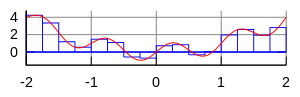
\includegraphics[width=6cm]{figs/Integration_rectangle.png}
\end{minipage}\\
where $w_{\mathrm{cell}}^{(t)}$ is the normalized probability of a grid cell $t$, and $\alpha^{(t)}$ and $\beta^{(t)}$ are center locations of grid cells
\end{itemize}
\item<2-> In 1D further variations with smaller error, e.g. trapezoid
  \begin{center}
    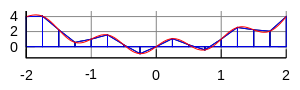
\includegraphics[width=6cm]{figs/Integration_trapezoid.png}
  \end{center}
\item<3-> In 2D and higher
  \begin{itemize}
  \item nested quadrature, product rules
  \item but theres a curse of dimensionality...
  \end{itemize}
  \end{itemize}


\end{frame}

\section{Monte Carlo Methods}

\begin{frame}


\frametitle{Monte Carlo integration/method}

  \begin{itemize}
    \item Numerically (deterministic) compute an integral (midpoint) using $S$ sample points
    \[
      I^a_b(h) = \int^a_b h(\theta) d\theta \approx \sum_s^S h(\theta_s) \frac{w_s}{S}
    \]
    where
    \[
    w_s = b - a
    \]
    and
    \[
    \theta_i = a - (s + 0.5) \delta\theta
    \]
    \pause
    \item In Gelman et al (2013) notation and for a posteriors $p(\theta|y)$
    \[
      E_{p(\theta|y)}(h(\theta)) = \int h(\theta) p(\theta|y) d\theta \approx \sum_s^S h(\theta_s) p(\theta_s|y) \frac{w_s}{S}
    \]
    \pause
    \item If we have samples $\theta_s \sim p(\theta|y)$ we can approximate
        \[
      E_{p(\theta|y)}(h(\theta)) = \int h(\theta) p(\theta|y) d\theta \approx \frac{1}{S} \sum_s^S h(\theta_s)
    \]
  \end{itemize}

\end{frame}

%    A (stochastic) numerical technique to approximate integrals
%    \item Main benefit: The error is $n^{-1/2}$ irrespective of dimension
%    \pause
%    \item Let $\theta \sim p(\theta)$, then
%    \[
%    E(g(\theta)) = \int g(\theta) p(\theta) d\theta
%    \]
%    \item

\begin{frame}
\frametitle{Monte Carlo - history}

  \begin{itemize}
  \item Used already before computers
    \begin{itemize}
      \item Buffon (18th century; needles)
      \item De Forest, Darwin, Galton (19th century)
      \item Pearson (19th century; roulette)
      \item Gosset (Student, 1908; hat)
    \end{itemize}
    \pause
  \item "Monte Carlo method" term was proposed by Metropolis, von Neumann
    or Ulam in the end of 1940s
     \begin{itemize}
     \item they worked together in atomic bomb project
     \item Metropolis and Ulam, "The Monte Carlo Method", 1949
     \end{itemize}
    \pause
   \item Bayesians started to have enough cheap computation time in 1990s
     \begin{itemize}
     \item BUGS project started 1989 (last OpenBUGS release 2014)
     \item Gelfand \& Smith, 1990
     \item Stan initial release 2012
     \end{itemize}
     % \begin{itemize}
     %   \item tätä ennen käyttö vähäistä, vaikka bayesilaisiakin
     %     osallistui teorian ja menetelmien kehittämiseen
     % \end{itemize}
  \end{itemize}

\end{frame}


\begin{frame}

\frametitle{Monte Carlo}

  \begin{itemize}
  \item Simulate draws from the target distribution $p(\theta|y)$
    \begin{itemize}
    \item these draws can be treated as any observations
    \item a collection of draws is a sample of size $S$
    \end{itemize}
  \item Use these draws, for example,
    \begin{itemize}
    \item to compute means, deviations, quantiles
    \item to draw histograms
    \item to marginalize
    \item etc.
    \end{itemize}
  \end{itemize}

\end{frame}

\begin{frame}


\frametitle{Monte Carlo vs. Deterministic Methods}

  \begin{itemize}
  \item Monte Carlo (approximation) error is $\propto S^{-1/2}$
  \item Midpoint rule error is $\propto S^{-2}$
  \item Trapezoidal rule error is $\propto S^{-2}$
  \item Simpson rule error is $\propto S^{-4}$
  \item Monte Carlo is bad (even worse than midpoint approximation)
  \only<1>{{\color{uured}Why use Monte Carlo integration?}}
  \pause
  \item Monte Carlo has the same error irrespective of dimension $D$, i.e. $S_D = S$
  \item Numerical methods create a grid with $S_D = S^D$
  \only<2>{{\color{uured} When is Monte Carlo a better approach than Simpsons?}}
  \pause
  \[
  (S_D^\frac{1}{D})^{-4} = S_D^{-\frac{1}{2}}\,,
  \]
  i.e. for $d > 8$ Monte Carlo is better.
  \end{itemize}

\end{frame}

\begin{frame}


\frametitle{How many simulation draws are needed?}

  \begin{itemize}
  \item How many draws or how big sample size $S$?
  \item If draws are independent
    \begin{itemize}
    \item usual methods to estimate the uncertainty due to a finite
      number of observations (finite sample size)
    \end{itemize}
  \item Markov chain Monte Carlo produces dependent draws (next week)
    \begin{itemize}
    \item requires additional work to estimate the \emph{effective
        sample size}
    \end{itemize}
  \end{itemize}

\end{frame}

\begin{frame}

\frametitle{How many simulation draws are needed?}

  \begin{itemize}
  \item Expectation of unknown quantity
    \begin{equation*}
      \E(\theta)\approx \frac{1}{S}\sum_{s=1}^S \theta^{(s)}
    \end{equation*}
    if $S$ is big and $\theta^{(s)}$ are independent, way may assume
    that the distribution of the expectation approaches normal
    distribution (see Ch 4) with variance $\sigma^2_\theta/S$
    (asymptotic normality)
    \begin{itemize}
    \item this variance is independent on dimensionality of $\theta$ (!)
      \pause
    \item total variance is sum of the epistemic uncertainty in the
      posterior and the uncertainty due to using finite number of
      Monte Carlo draws
      \begin{equation*}
        \sigma^2_\theta+\sigma^2_\theta/S \pause= \sigma^2_\theta(1+1/S)
      \end{equation*}
      \pause
      \vspace{-5mm}
    \item e.g. if $S=100$, deviation increases by $\sqrt{1+1/S}=1.005$\\
      i.e. Monte Carlo error is very small (for the expectation)
      \pause
    \item See Ch 4 for counter-examples for asymptotic normality
    \end{itemize}
\end{itemize}

\end{frame}

\begin{frame}

\frametitle{Example: Kilpisjärvi summer temperature}

  Average temperature in June, July, and August at Kilpisjärvi, Finland

  \begin{center}
    \only<1>{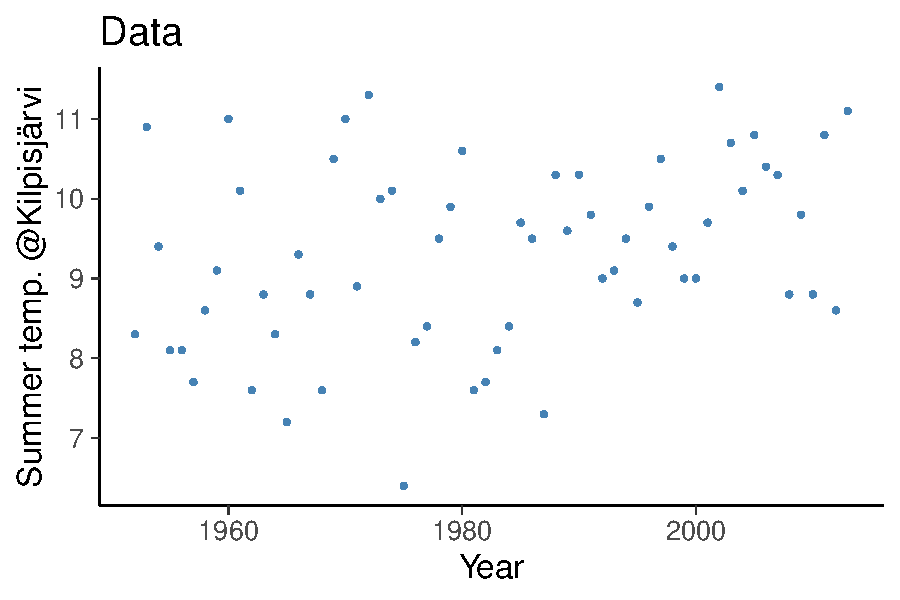
\includegraphics[width=8cm]{figs/kilpis_data.pdf}}
    \only<2>{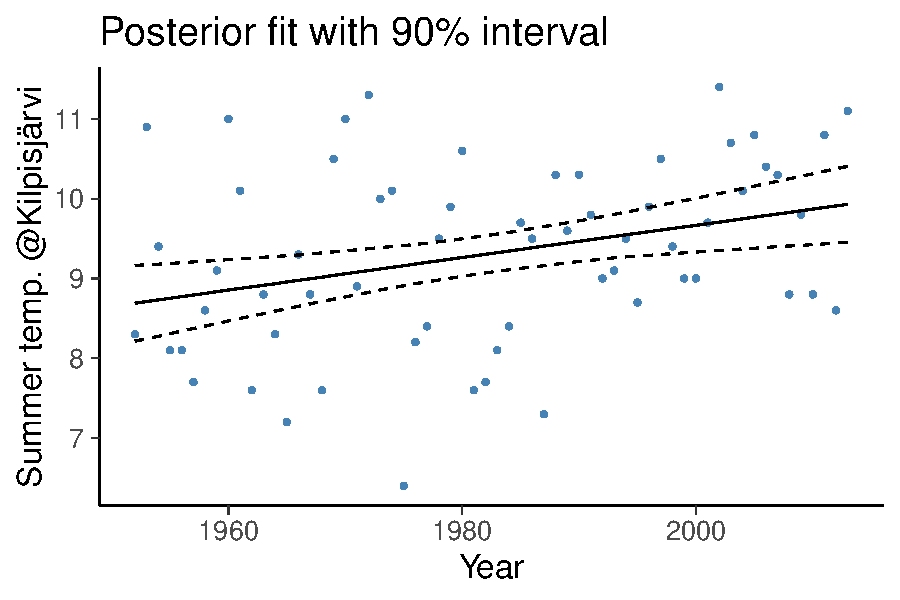
\includegraphics[width=8cm]{figs/kilpis_pfit.pdf}}
  \end{center}

\end{frame}

\begin{frame}

\frametitle{Example: Kilpisjärvi summer temperature}

  \begin{center}
    \only<1>{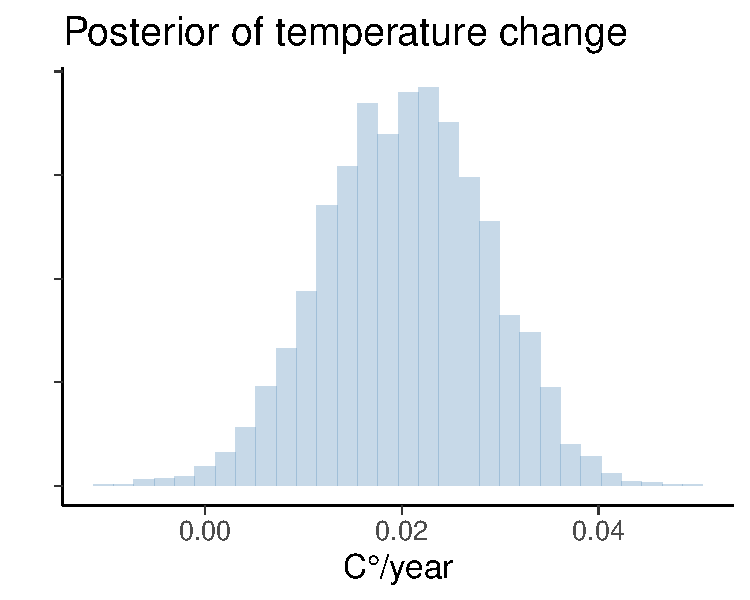
\includegraphics[width=8cm]{figs/kilpis_phist.pdf}}
    \only<2>{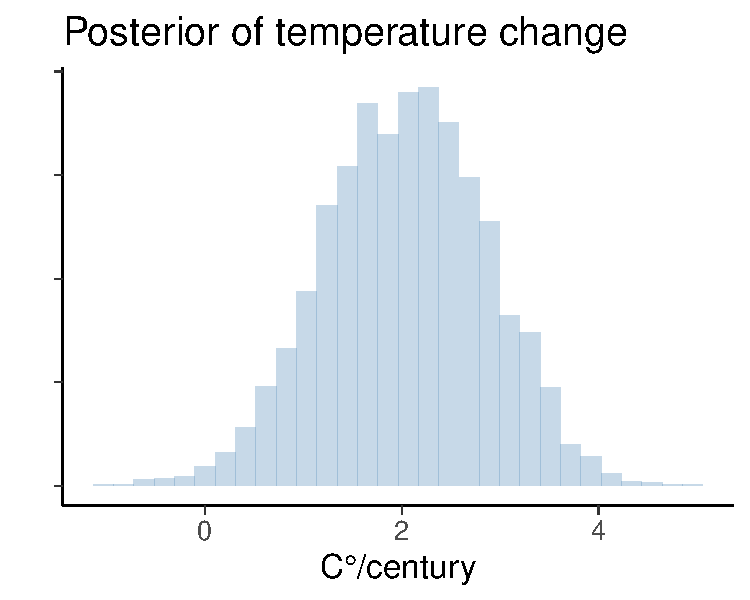
\includegraphics[width=8cm]{figs/kilpis_phist100.pdf}}
    \only<3>{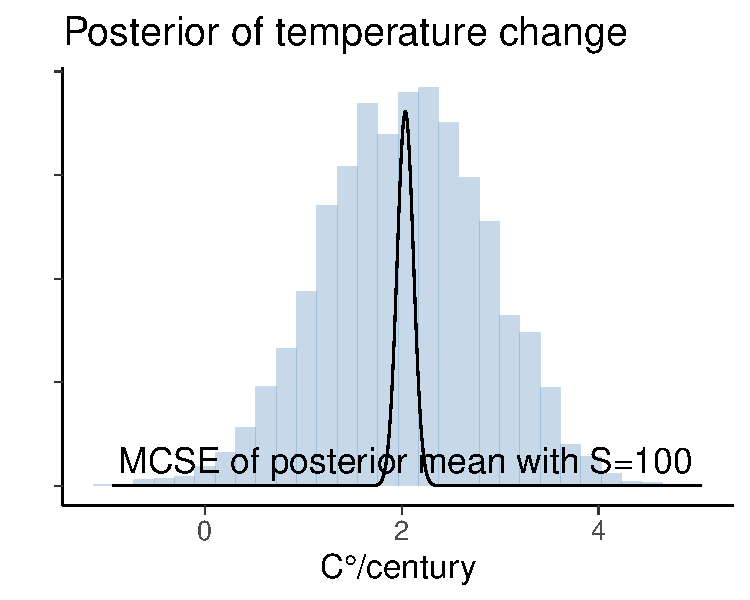
\includegraphics[width=8cm]{figs/kilpis_phist100_mcse1a.pdf}}
    \only<4>{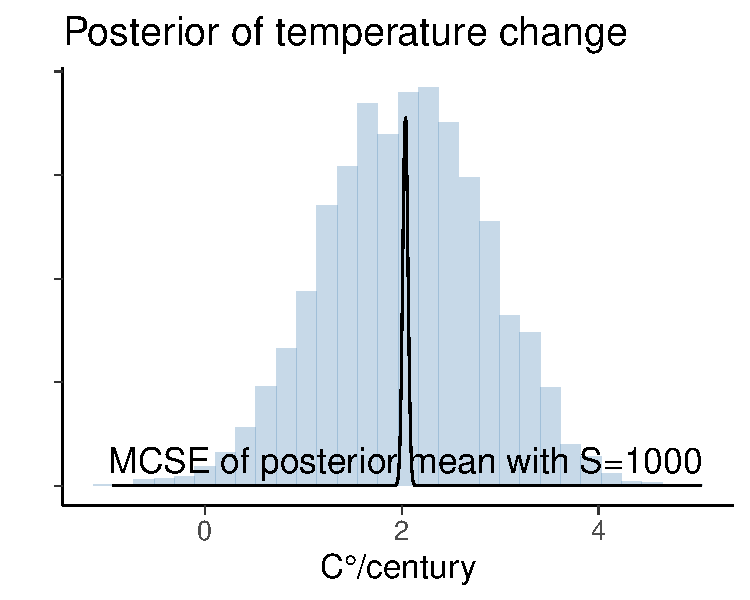
\includegraphics[width=8cm]{figs/kilpis_phist100_mcse1b.pdf}}
    \only<3>{$\sigma_\theta\approx 0.827,\, \text{MCSE} \approx 0.0827,\, \text{total deviation} \approx 0.831$\\}
    \only<4>{$\sigma_\theta\approx 0.827,\, \text{MCSE} \approx 0.0261,\, \text{total deviation} \approx 0.827$\\}
     \uncover<3-4>{\vspace{0.5\baselineskip}\color{gray} $\text{total deviation}^2 = \sigma_\theta^2 + \text{MCSE}^2$}
  \end{center}

\end{frame}

\begin{frame}

\frametitle{Example: Kilpisjärvi summer temperature}

  \vspace{\baselineskip}
  \makebox[10cm][t]{
    \hspace{-0.9cm}
  \begin{minipage}[b][10cm][t]{10cm}
    \only<1->{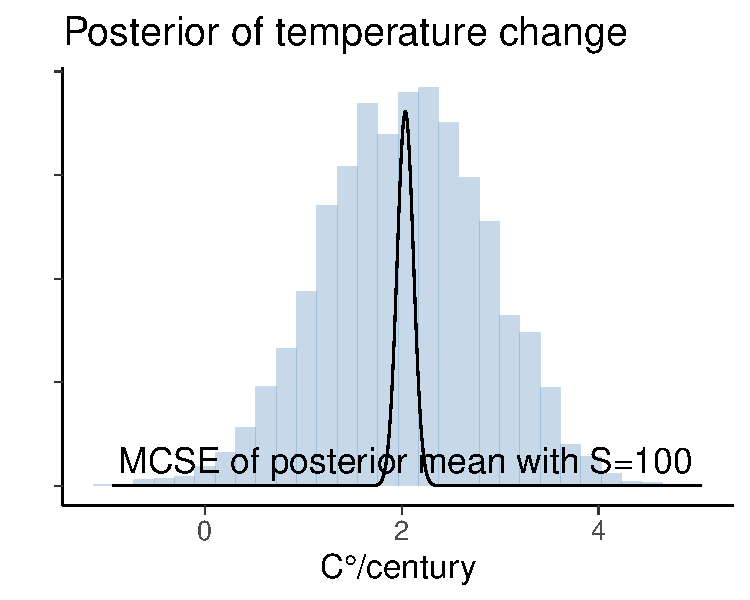
\includegraphics[width=3cm]{figs/kilpis_phist100_mcse1a.pdf}}
    \only<2->{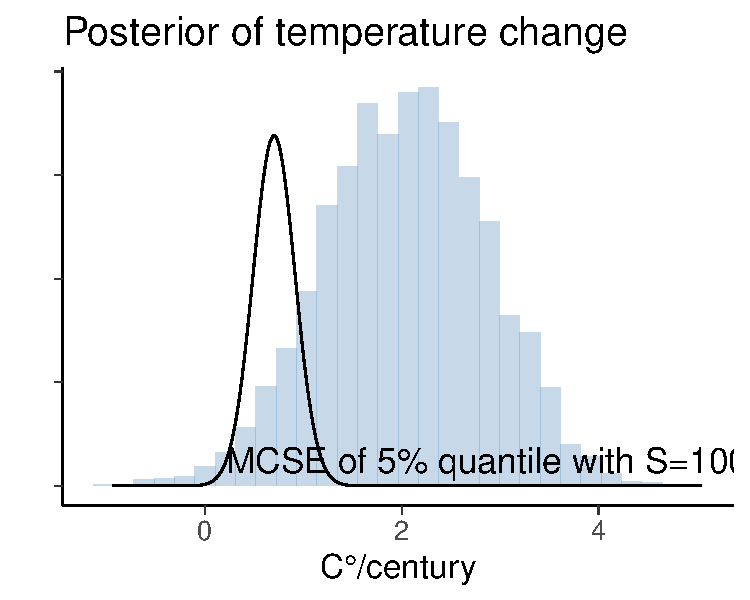
\includegraphics[width=3cm]{figs/kilpis_phist100_mcse2a.pdf}}
    \only<3->{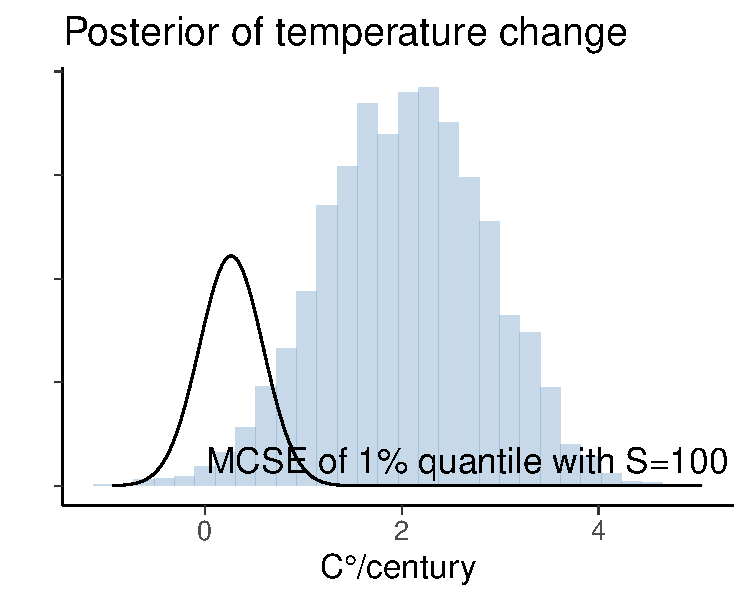
\includegraphics[width=3cm]{figs/kilpis_phist100_mcse3a.pdf}}\\
    \only<1->{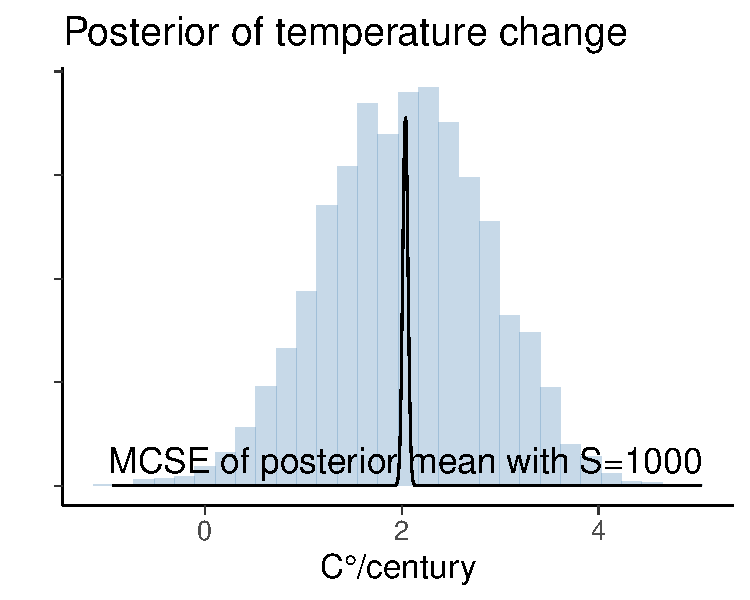
\includegraphics[width=3cm]{figs/kilpis_phist100_mcse1b.pdf}}
    \only<2->{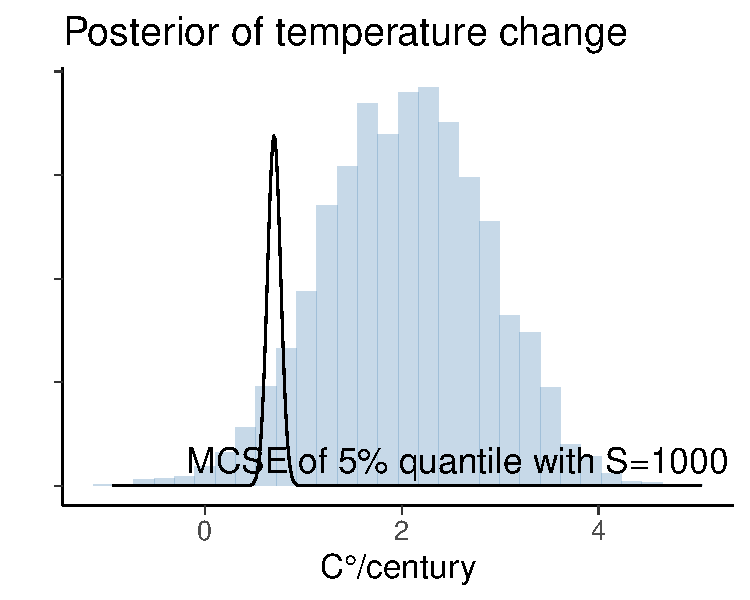
\includegraphics[width=3cm]{figs/kilpis_phist100_mcse2b.pdf}}
    \only<3->{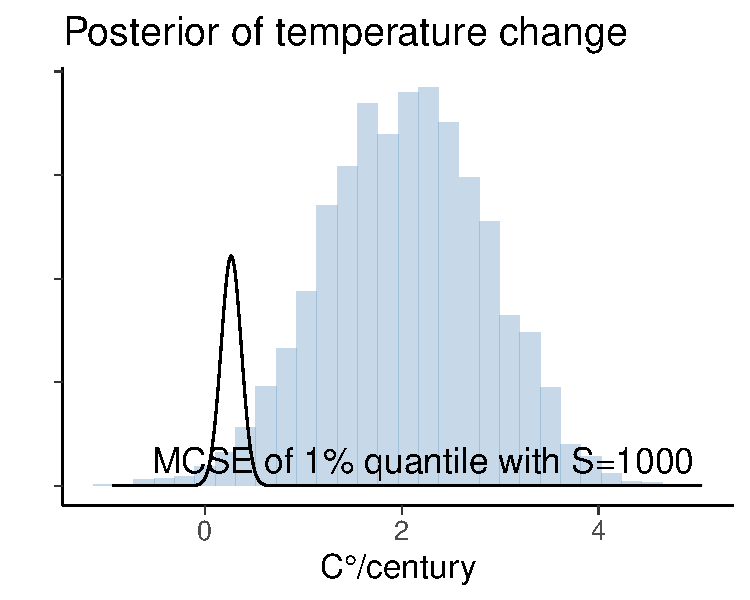
\includegraphics[width=3cm]{figs/kilpis_phist100_mcse3b.pdf}}\\
    \begin{center}
      \vspace{-\baselineskip}
  \only<4->{Tail quantiles are more difficult to estimate}
\end{center}
  \end{minipage}
  }

\end{frame}

\begin{frame}

\frametitle{How many simulation draws are needed?}

  \begin{itemize}
  \item Posterior probability
    \begin{equation*}
      p(\theta \in A)\approx \frac{1}{S}\sum_l I(\theta^{(s)} \in A)
    \end{equation*}
    where $I(\theta^{(s)} \in A)=1$ if $\theta^{(s)} \in A$
    \begin{itemize}
    \pause
    \item $I(\cdot)$ is binomially distributed as $p(\theta \in A)$
        \begin{itemize}
        \item[$\rightarrow$] $\var(I(\cdot)) =  p(1-p)$  (Appendix A, p. 579)
        \item[$\rightarrow$] standard deviation of $p$ is $\approx \sqrt{p(1-p)/S}$
        \end{itemize}
        \pause
      \item if $S=100$ and $p\approx 0.5$, $\sqrt{p(1-p)/S}=0.05$\\
        i.e. accuracy is about $5\%$ units
        \pause
      \item $S=2500$ draws needed for $1\%$ unit accuracy
    \end{itemize}
    \pause
  \item To  estimate small probabilities, a large number of draws is needed
    \begin{itemize}
    \item to be able to estimate $p$, need to get draws with
      $\theta^{(l)} \in A$, which in expectation requires $S \gg 1/p$
    \end{itemize}
\end{itemize}

\end{frame}

\begin{frame}

\frametitle{Example: Kilpisjärvi summer temperature}

  \begin{center}
    \only<1>{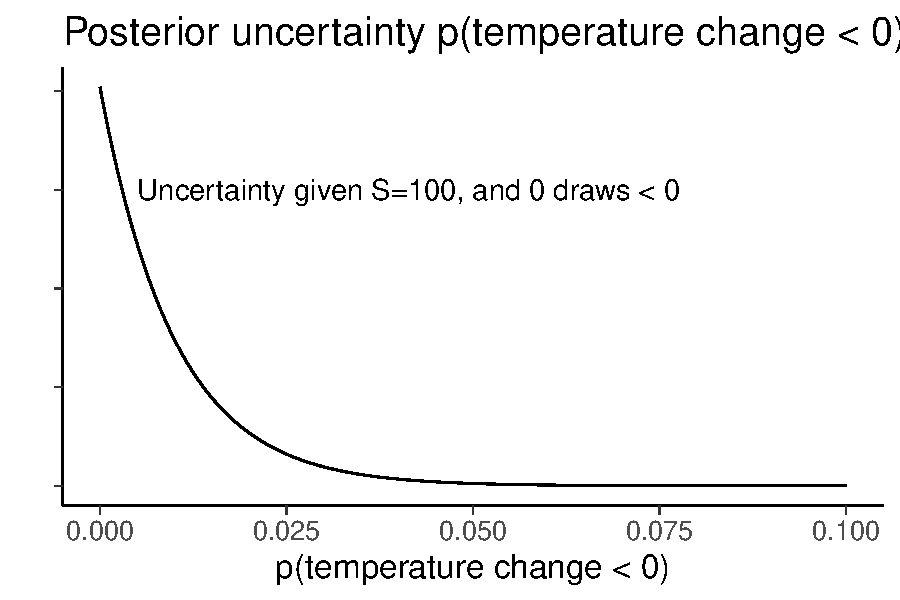
\includegraphics[width=8cm]{figs/kilpis_ppneg_mcse1a.pdf}}
    \only<2>{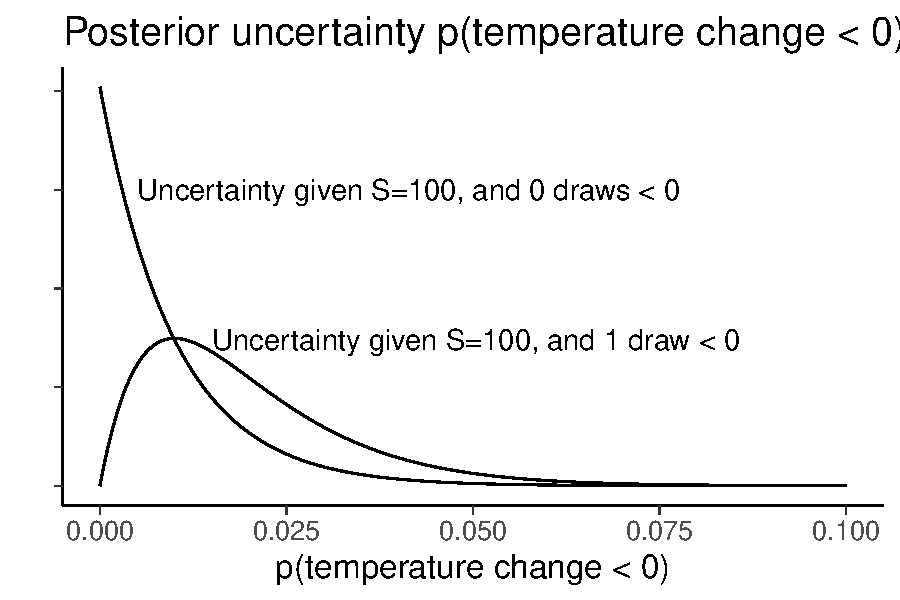
\includegraphics[width=8cm]{figs/kilpis_ppneg_mcse1b.pdf}}
    \only<3>{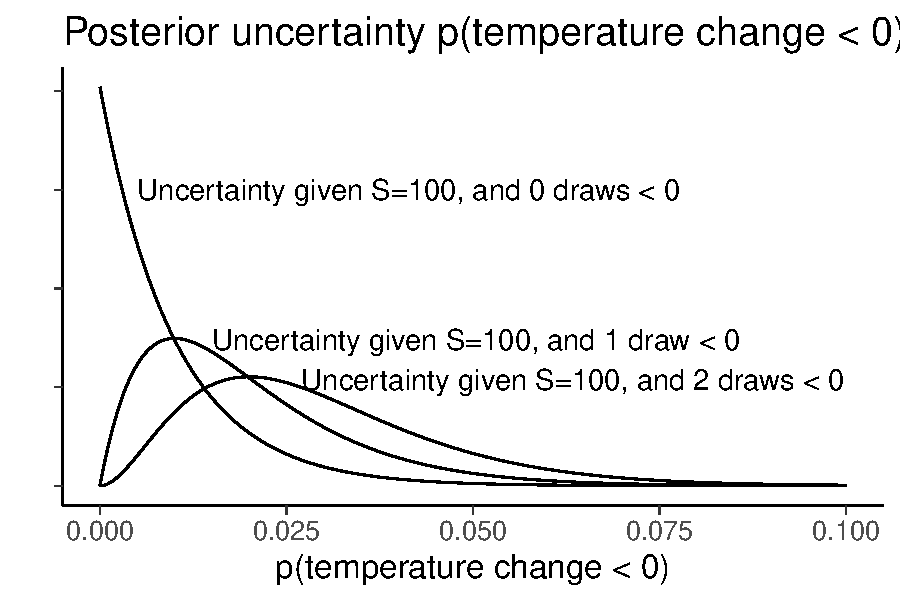
\includegraphics[width=8cm]{figs/kilpis_ppneg_mcse1c.pdf}}
    \only<4>{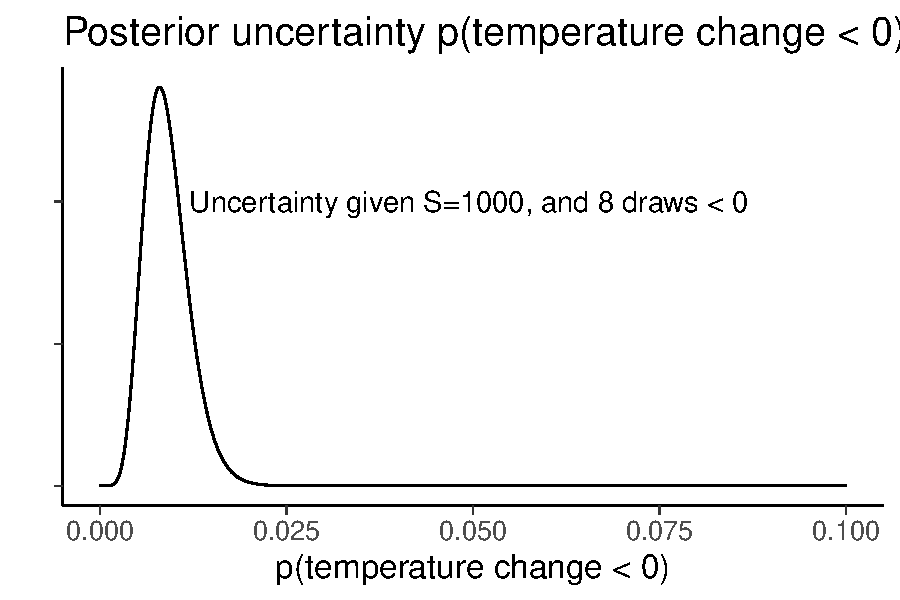
\includegraphics[width=8cm]{figs/kilpis_ppneg_mcse1000.pdf}}
    \only<5>{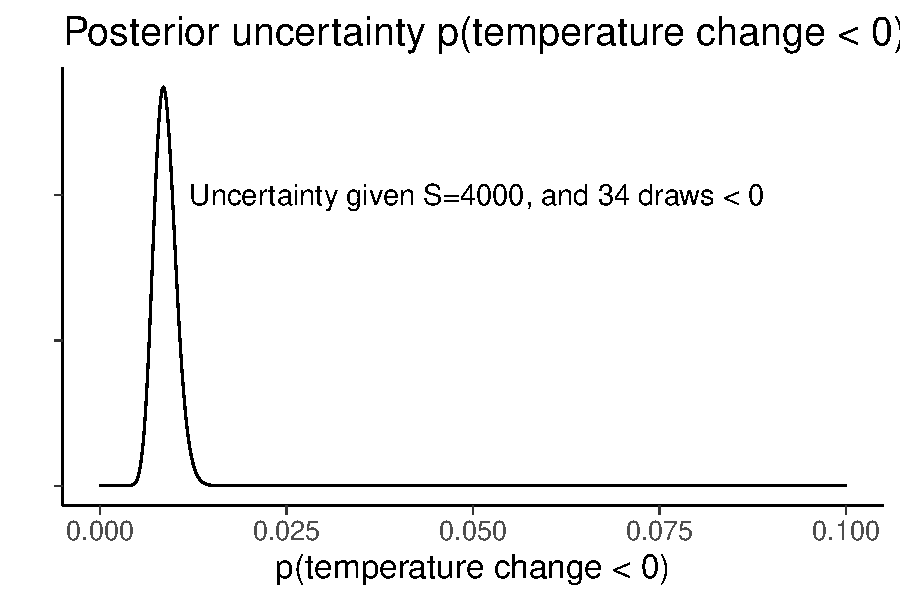
\includegraphics[width=8cm]{figs/kilpis_ppneg_mcse4000.pdf}}
  \end{center}

\end{frame}

\begin{frame}

\frametitle{How many digits to show in reports?}


  \begin{itemize}
  \item Too many digits make reading of the results slower and give
    false impression of the accuracy
  \item<2-> Don't show digits which are just random noise
    \begin{itemize}
    \item check what is the Monte Carlo standard error
    \end{itemize}
  \item<3-> Show meaningful digits given the posterior uncertainty
  \item<4-> Example: The mean and 90\% central posterior interval for temperature
     increase C$^\circ$/century based on posterior draws
     \begin{itemize}
     \item<5-> {\color{red} 2.050774 and $[$0.7472868 3.3017524$]$} (NO!)
     \item<6-> {\color{uured} 2.1 and $[$0.7 3.3$]$}
    \item<7-> {\color{uured} 2 and $[$1 3$]$} (depends on the context)
     \end{itemize}
   \item<8-> Example: The probability that temp increase is
     positive
     \begin{itemize}
     \item<9-> {\color{red} 0.9960000} (NO!)
     \item<10-> {\color{uured} 1.00} (depends on the context)
     \item<11-> With 4000 draws MCSE $\approx$ 0.002. We could report
       that probability is {\color{uured} very likely larger than 0.99}, or sample
       more to justify reporting three digits
     \item<12-> For probabilities close to 0 or 1, consider also when
       the model assumption justify certain accuracy
     \end{itemize}
   \item<12-> For your project: Think for each reported value how many digits is sensible.
  \end{itemize}

\end{frame}


\begin{frame}

\frametitle{How many simulation draws are needed?}

  \begin{itemize}
  \item Less draws needed with
    \begin{itemize}
    \item deterministic methods
    \item marginalization (Rao-Blackwellization)
    \item variance reduction methods, such, control variates
    \end{itemize}
  \end{itemize}

\end{frame}

\begin{frame}

\frametitle{How many simulation draws are needed?}

  \begin{itemize}
  \item Number of independent draws needed doesn't depend on the number of dimensions
    \begin{itemize}
    \item but it may be difficult to obtain independent draws in high dimensional case
    \end{itemize}
  \end{itemize}

\end{frame}

\begin{frame}

\section{Direct sampling}

\frametitle{Direct sampling}

  \begin{itemize}
  \item Direct simulation from known pdf/pmf, e.g. $p(\theta|y)$ in conjugate case
  \item Produces independent draws
    \begin{itemize}
    \item Using analytic transformations of uniform random numbers
      (e.g. appendix A)
    \item factorization
    \item numerical inverse-CDF
    \end{itemize}
  \item {\color{uured} Problem}: restricted to limited set of models
  \end{itemize}

\end{frame}

\begin{frame}

\frametitle{Random number generators}

  \begin{itemize}
  \item {\color{uured}How to sample from a pdf?}
  \pause
  \item Good {\color{uured} psuedo} random number generators are sufficient for Bayesian inference
  \begin{itemize}
    \item pseudo random generator uses deterministic algorithm to
      produce a sequence which is difficult to make difference from
      truly random sequence
    \item modern software used for statistical analysis have good
      pseudo RNGs
    \end{itemize}
  \end{itemize}

\end{frame}

\begin{frame}


\frametitle{Direct simulation: Example}

  \begin{itemize}
  \item Box-Muller -method:\\ If $U_1$ and $U_2$ are independent
    draws from distribution $\U(0,1)$, and
    \begin{align*}
      X_1 & = \sqrt{-2\log(U_1)}\cos(2\pi U_2) \\
      X_2 & = \sqrt{-2\log(U_1)}\sin(2\pi U_2)
    \end{align*}
    then $X_1$ and $X_2$ are independent draws from the distribution
    $\N(0,1)$
    \pause
    \begin{itemize}
      \item not the fastest method due to trigonometric computations
      \item for normal distribution more than ten different methods
      \item e.g. R uses inverse-CDF
    \end{itemize}
  \end{itemize}

\end{frame}


\begin{frame}
\frametitle{Grid sampling and curse of dimensionality}

  \begin{itemize}
      \item 10 parameters
      \item if we don't know beforehand where the posterior mass is
        \begin{itemize}
          \item need to choose wide box for the grid
          \item need to have enough grid points to get some of them
            where essential mass is
        \end{itemize}
      \only<1>{{\color{uured} Can we do this?}}
      \item e.g. 50 or 1000 grid points per dimension
        \begin{itemize}
        \item[$\rightarrow$] 50$^{10} \approx$ 1e17 grid points
        \item[$\rightarrow$] 1000$^{10} \approx$ 1e30 grid points
        \end{itemize}
      \pause
      \item R and my current laptop can compute density of normal
        distribution about 20 million times per second
        \begin{itemize}
        \item[$\rightarrow$] evaluation in 1e17 grid points would take
           150 years %triljoona vuotta
        \item[$\rightarrow$] evaluation in 1e30 grid points would take
           1 500 billion years %triljoona vuotta
        \end{itemize}
 \end{itemize}

\end{frame}

\section{Indirect sampling}

\begin{frame}

\frametitle{Indirect sampling}

  \begin{itemize}
  \item Rejection sampling
    % \begin{itemize}
    % \item draw directly from a proposal distribution, reject some
    %   draws, remaining draws are independent draws from the target
    %   distribution
    % \end{itemize}
    % \pause
  \item Importance sampling
    % \begin{itemize}
    % \item draw directly from a proposal distribution, weight the draws
    % \end{itemize}
    % \pause
  \item Markov chain Monte Carlo (next week)
    % \begin{itemize}
    % \item draw directly from a transition distribution forming a
    %   Markov chain, draws are dependent draws from the target
    %   distribution
    % \end{itemize}
  \end{itemize}

\end{frame}

\begin{frame}

\frametitle{Effective sampling size}

  \begin{itemize}
    \item Efficient sampling size $S_\text{eff}$ the number of samples using direct methods
    \item Common with {\color{uured} weighted} or {\color{uured} correlated} samples
    \pause
    \item Indirect methods usually have an $S_\text{eff} < S$
    \item Informally an indication of performance of method
  \end{itemize}

\end{frame}

\subsection{Rejection sampling}

\begin{frame}

\frametitle{Rejection sampling}

    \vspace{-.3\baselineskip}
  \begin{itemize}
  \item[-] Proposal ($g(\theta)$) forms envelope over the target distribution ${q(\theta|y)}/{M g(\theta)} \leq 1$
  \item[-] Draw from the proposal and accept with probability ${q(\theta|y)}/{M g(\theta)}$
  \item<3>[-] Common for truncated distributions
  \end{itemize}

  \begin{center}
    \vspace{-1.6\baselineskip}
    \only<1>{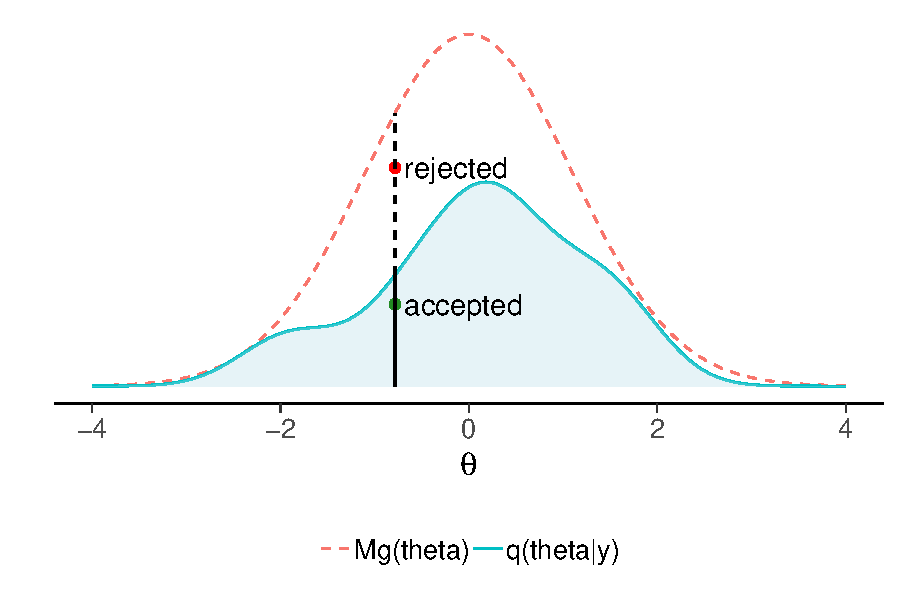
\includegraphics[width=8cm]{figs/rejection1.pdf}}
    \only<2>{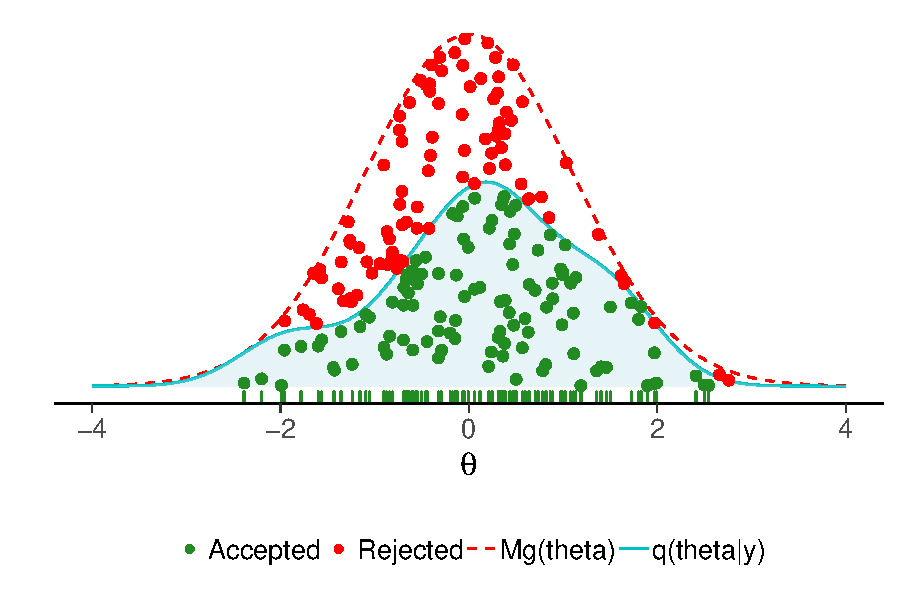
\includegraphics[width=8cm]{figs/rejection2.pdf}}
    \only<3>{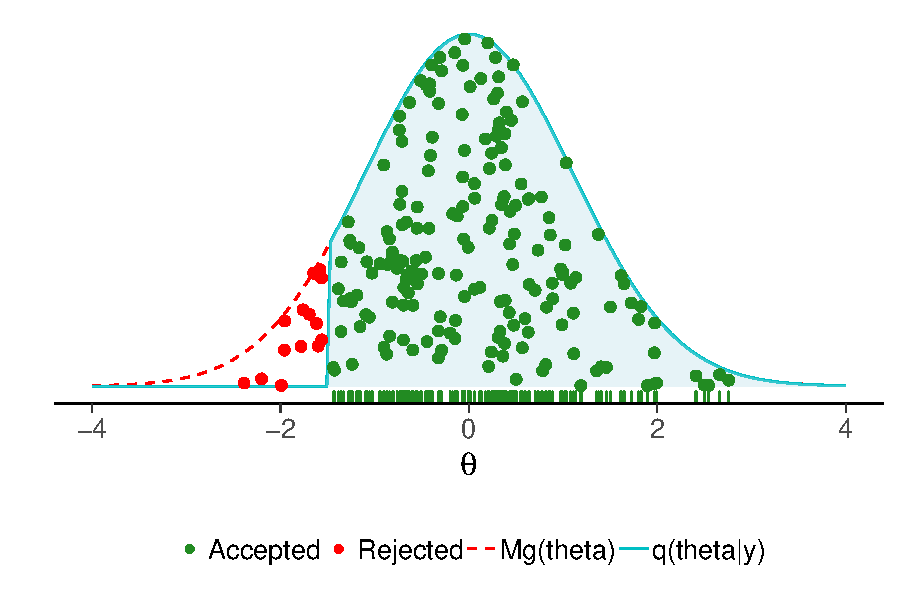
\includegraphics[width=8cm]{figs/rejection3.pdf}}
  \end{center}

\end{frame}

\begin{frame}
\frametitle{Rejection sampling}

\begin{itemize}
  \item The number of accepted draws is the effective sample size $S_\text{eff}$

  \only<1>{{\color{uured} When will this be work/not work (i.e. give high/low $S_\text{eff}$)?}}
  \pause
    \begin{itemize}
    \item with bad proposal distribution may require a lot of trials
    \item selection of good proposal gets very difficult when
      the number of dimensions increase
%      \pause
%    \item reliable diagnostics and thus can be a useful part
    \end{itemize}
  \end{itemize}

\end{frame}

\subsection{Importance sampling}

\begin{frame}

\frametitle{Importance sampling}

  \begin{itemize}
     \vspace{-.5\baselineskip}
   \item[-] Proposal does not need to have a higher value everywhere
   \end{itemize}
   \begin{center}
     \vspace{-1\baselineskip}
     \only<1-2>{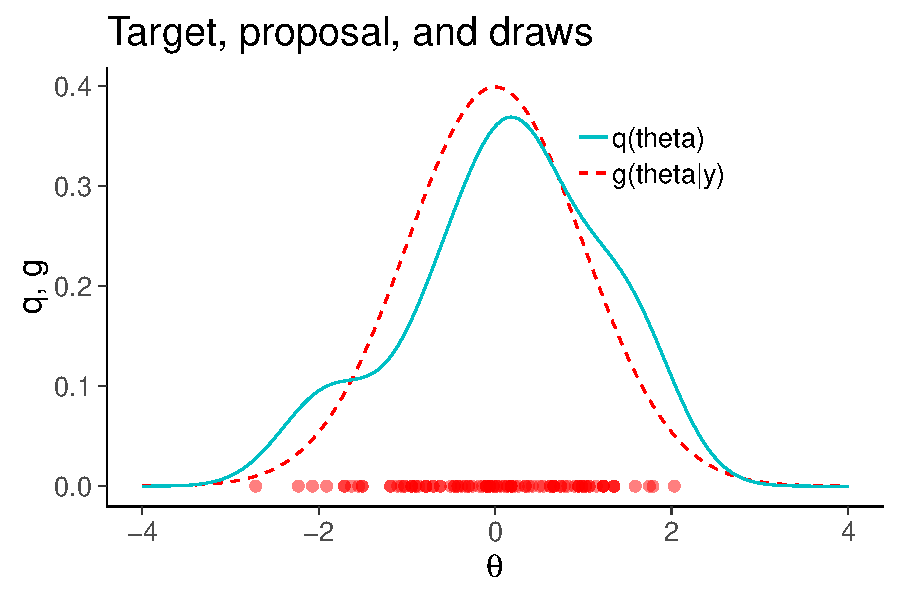
\includegraphics[width=9cm]{figs/importancesamp1.pdf}}
     \only<3>{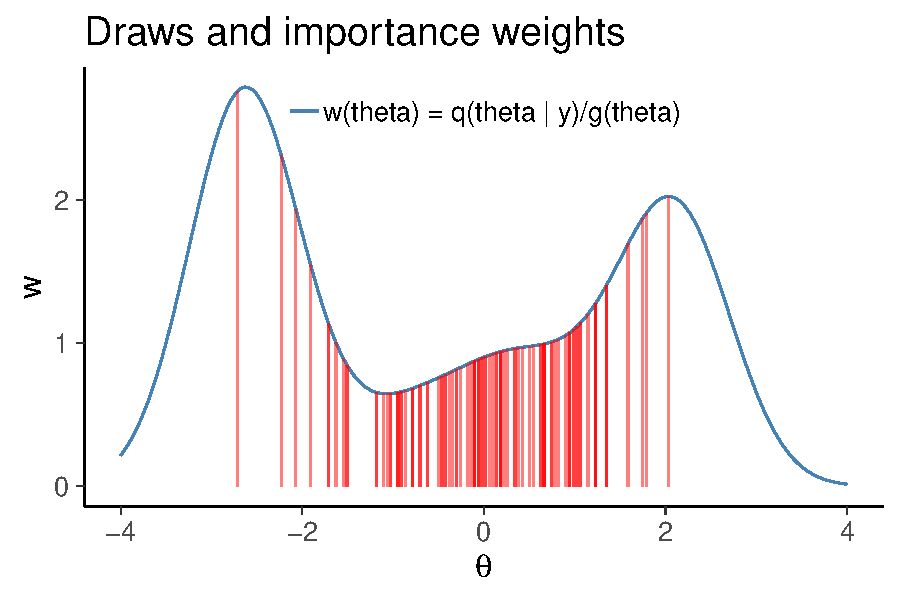
\includegraphics[width=9cm]{figs/importancesamp2.pdf}}
     \vspace{-1\baselineskip}
     \only<2->{
   \begin{eqnarray*}
      \E[f(\theta)] \approx \frac{\sum_s w_s f(\theta^{(s)})}{\sum_s
      w_s}, \qquad \text{where} \quad
      w_s =  \frac{q(\theta^{(s)})}{g(\theta^{(s)})} \qquad
   \end{eqnarray*}
   }
   \end{center}

\end{frame}

\begin{frame}

\frametitle{Importance sampling}

  \begin{itemize}
  \item Resampling using normalized importance weights can be used to
    pick a smaller number of draws with uniform weights
    \pause
  \item Selection of good proposal gets more difficult when the
      number of dimensions increase
      \pause
    \item Often used to correct distributional approximations and leave-one-out cross-validation
  \end{itemize}

\end{frame}

\begin{frame}

\frametitle{Importance sampling}

  \begin{itemize}
  \item Variation of the weights affect the {\color{uured} effective sample size}
    \begin{itemize}
    \item if single weight dominates, we have effectively one sample
    \item if all weights are equal, we have effectively $S$ draws
    \end{itemize}
    \only<1>{{\color{uured}What does this mean? What is a good proposal $g(\theta)$?}}
    \pause
  \item Central limit theorem holds only if variance of the weight
    distribution is finite
%  \item See Vehtari, Simpson, Gelman, Yuling and Gabry (2019). Pareto
%    smoothed importance sampling. arXiv preprint arXiv:1507.02646,
%    \url{https://arxiv.org/abs/1507.02646} for improved diagnostics
%    and stability.
  \end{itemize}

\end{frame}

\begin{frame}

\frametitle{Example: Importance sampling in Bioassay}

   \vspace{-.5\baselineskip}
   \makebox[9cm][t]{
     \hspace{-0.9cm}
     \begin{minipage}[t][12cm][t]{12cm}
       \begin{center}
        \makebox[0cm][t]{\hspace{-0.5cm}\rotatebox{90}{\hspace{1cm}Grid}}
        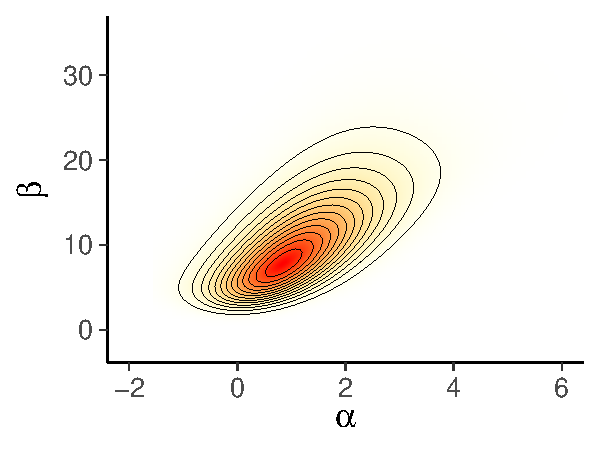
\includegraphics[width=2.5cm]{figs/bioassayis1d.pdf}
      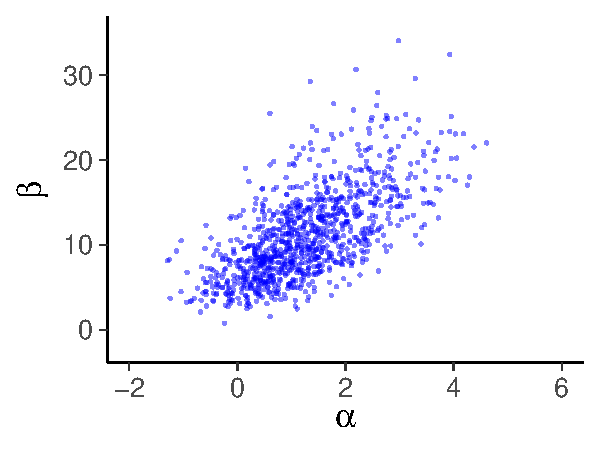
\includegraphics[width=2.5cm]{figs/bioassayis1s.pdf}
      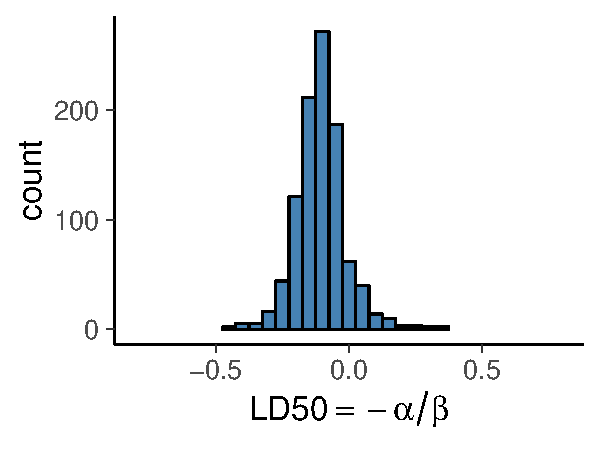
\includegraphics[width=2.5cm]{figs/bioassayis1h.pdf}\\
      \only<2->{
        \makebox[0cm][t]{\hspace{-0.5cm}\rotatebox{90}{\hspace{1cm}Normal}}
      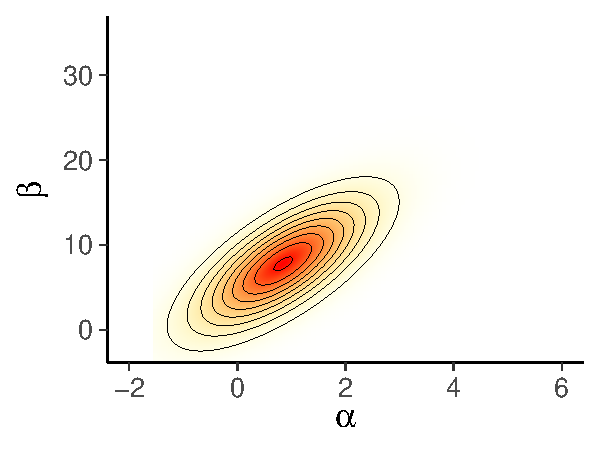
\includegraphics[width=2.5cm]{figs/bioassayis2d.pdf}
      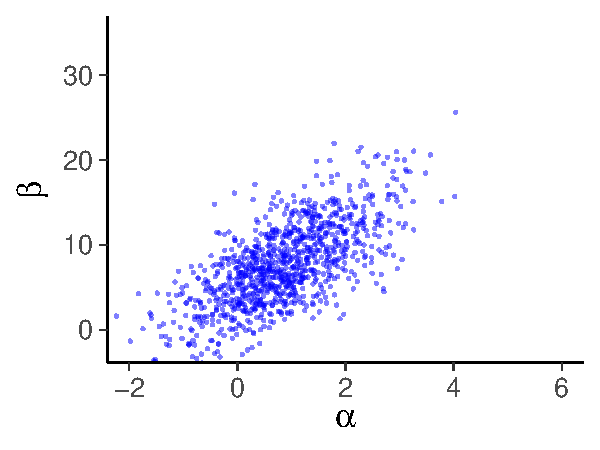
\includegraphics[width=2.5cm]{figs/bioassayis2s.pdf}
      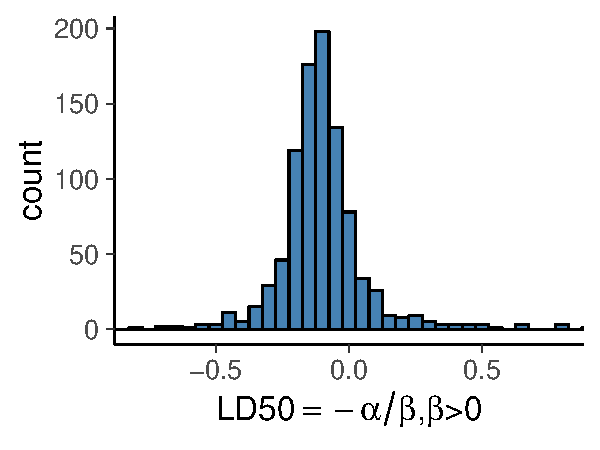
\includegraphics[width=2.5cm]{figs/bioassayis2h.pdf}\\}
    \only<2-3>{Normal approximation is discussed more in BDA3 Ch 4\\}
    \only<3>{But the normal approximation is not that good here:\\ Grid sd(LD50) $\approx$ 0.1, Normal sd(LD50) $\approx$ .75!}
      \only<4->{
        \makebox[0cm][t]{\hspace{-0.5cm}\rotatebox{90}{\hspace{1cm}IR}}
      
\includegraphics[width=2.5cm]{figs/bioassayis3d.pdf}
      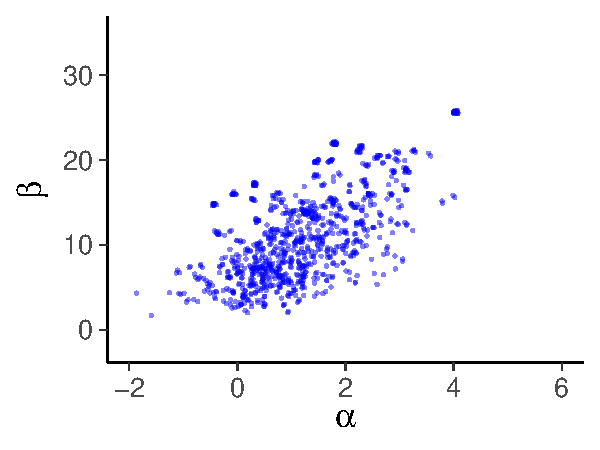
\includegraphics[width=2.5cm]{figs/bioassayis3s.pdf}
      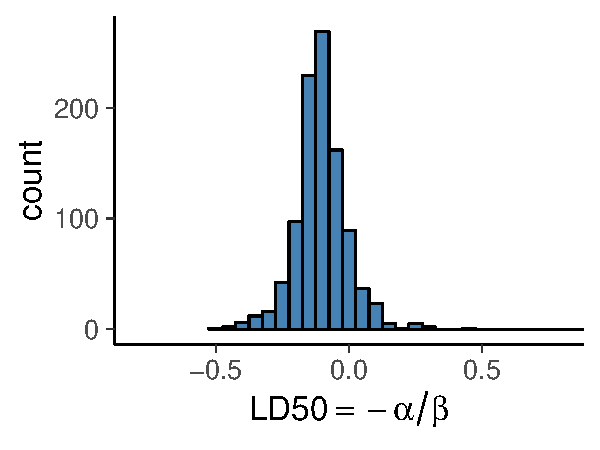
\includegraphics[width=2.5cm]{figs/bioassayis3h.pdf}\\}
    \only<5->{Grid sd(LD50) $\approx$ 0.1, IR sd(LD50) $\approx$ 0.1}
    \end{center}
     \end{minipage}
   }

\end{frame}

\begin{frame}

\frametitle{Example: Importance sampling in Bioassay}


   \makebox[8cm][t]{
     \hspace{-0.9cm}
     \begin{minipage}[t][4cm][t]{4cm}
       \begin{center}
       Grid\\
       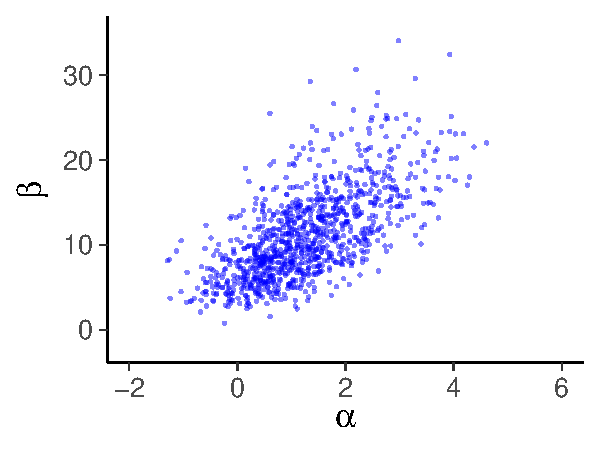
\includegraphics[width=4cm]{figs/bioassayis1s.pdf}
     \end{center}
     \end{minipage}
     \begin{minipage}[t][4cm][t]{4cm}
       \begin{center}
       IR\\
       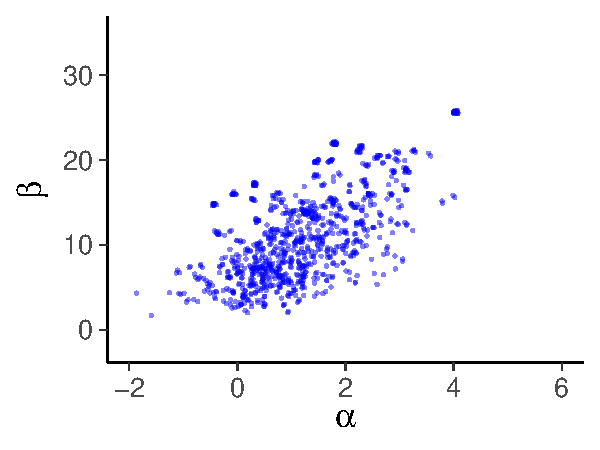
\includegraphics[width=4cm]{figs/bioassayis3s.pdf}
  \end{center}
  \end{minipage}
}

\end{frame}


\begin{frame}

\frametitle{Example: Importance sampling in Bioassay}

       \begin{center}
       IR\\
       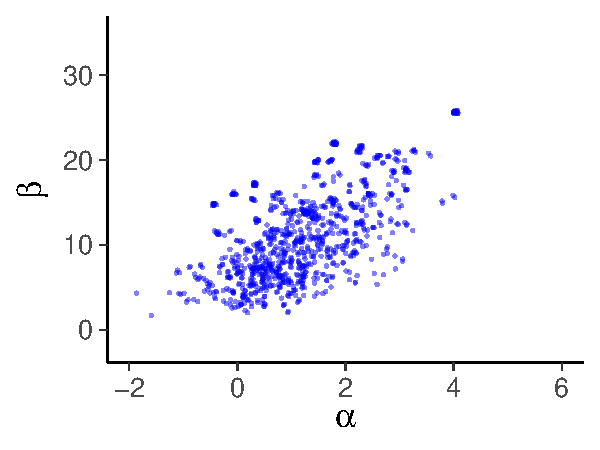
\includegraphics[width=8cm]{figs/bioassayis3s.pdf}
  \end{center}

\end{frame}

\begin{frame}

\frametitle{Example: Importance sampling in Bioassay}

       \begin{center}
       \only<1>{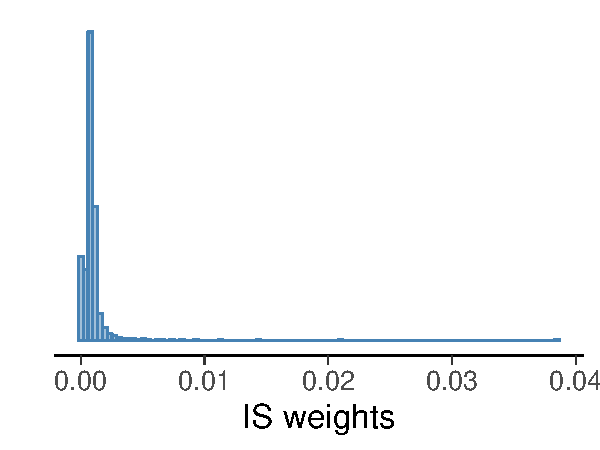
\includegraphics[width=8cm]{figs/bioassayisw1.pdf}}
       \only<2>{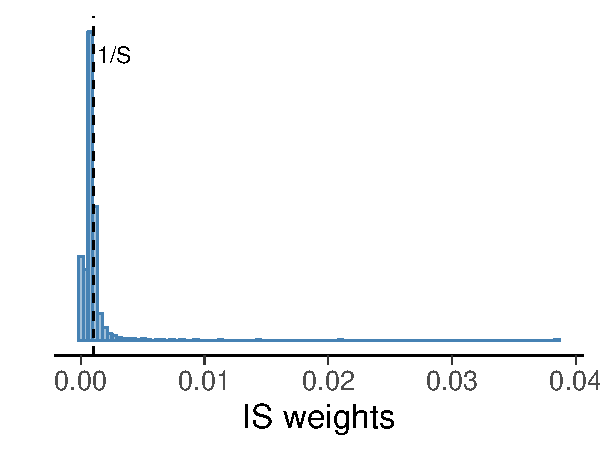
\includegraphics[width=8cm]{figs/bioassayisw2.pdf}}
       \only<3>{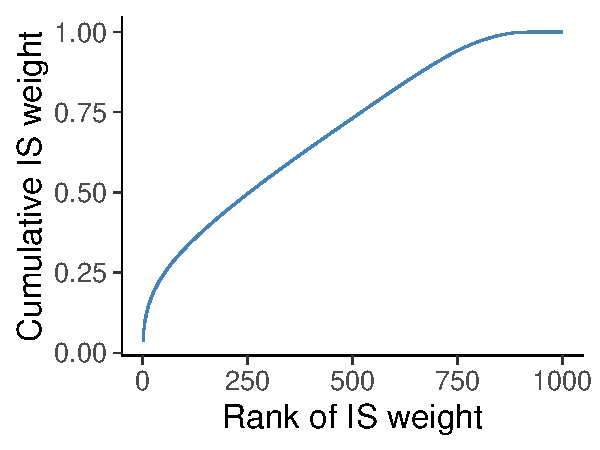
\includegraphics[width=8cm]{figs/bioassayisw3.pdf}}
  \end{center}

\end{frame}

\begin{frame}

\frametitle{Example: Importance sampling in Bioassay}
       \begin{center}
         \vspace{-\baselineskip}
       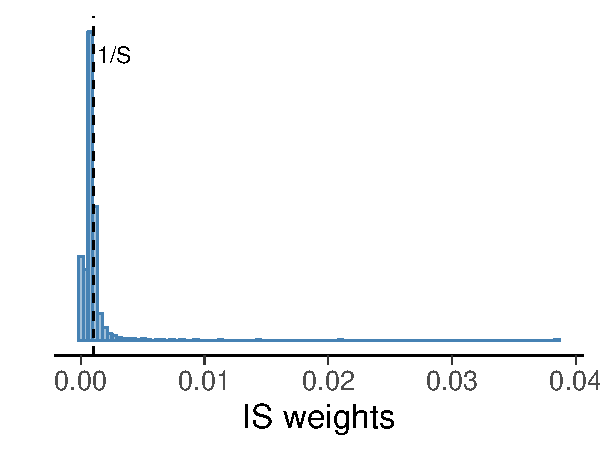
\includegraphics[width=8cm]{figs/bioassayisw2.pdf}\\
         \vspace{-2\baselineskip}
         \begin{align*}
           S_{\rm eff} & = \frac{1}{\sum_{s=1}^S (\tilde{w}(\theta^s))^2}, \quad \text{where } \tilde{w}(\theta^s)=w(\theta^s)/\sum_{s'=1}^Sw(\theta^{s'})\\
           \only<3->{S_{\rm eff} & \approx 270}
         \end{align*}
           \only<2>{{\color{red}
               \makebox[0cm][c]{\parbox{9.5cm}{\vspace{-2.5\baselineskip} \footnotesize BDA3 1st (2013) and 2nd (2014) printing have an error for $\tilde{w}(\theta^s)$. The normalized weights equation should not have the multiplier S (the normalized weights should sum to one). Errata for the book\\ \url{http://www.stat.columbia.edu/~gelman/book/errata_bda3.txt}\vspace{-2\baselineskip}}}}}
           \only<3>{\phantom{{\color{red}
            \makebox[0cm][c]{\parbox{9.5cm}{\vspace{-2.5\baselineskip} \footnotesize BDA3 1st (2013) and 2nd (2014) printing have an error for $\tilde{w}(\theta^s)$. The normalized weights equation should not have the multiplier S (the normalized weights should sum to one). Errata for the book\\ \url{http://www.stat.columbia.edu/~gelman/book/errata_bda3.txt}\vspace{-2\baselineskip}}}}}}
  \end{center}

\end{frame}




\subsection{Pareto-Smoothed Importance Sampling}

% TODO: Add more math here

\begin{frame}

\frametitle{Pareto smoothed importance sampling}

  \begin{itemize}
  \item Pareto-Smoothed Importance sampling smooth the weights according to a Generalized Pareto($k$) distribution
  \item Pareto-$k$ diagnostic estimate the number of existing moments ($\lfloor 1/k \rfloor$)
  \item<2-> Finite variance and central limit theorem for $k<1/2$
  \item<3-> Finite mean and generalized central limit theorem for $k<1$,
    but pre-asymptotic constant grows impractically large for $k>0.7$
  \end{itemize}
\end{frame}
% \\ \uncover<2->{&\text{Pareto-$k$ diagnostic preferably $<$ 0.7: }}\uncover<3->{ \hat{k} \approx 0.57}

\begin{frame}

\frametitle{Importance sampling leave-one-out cross-validation}

  \begin{itemize}
  \item Later in the course you will learn how $p(\theta|y)$ can be
    used as a proposal distribution for $p(\theta|y_{-i})$
    \begin{itemize}
    \item which allows fast computation of leave-one-out cross-validation
      \begin{align*}
        p(y_i|y_{-i})=\int p(y_i|\theta) p(\theta|y_{-i}) d\theta
      \end{align*}
    \end{itemize}
  \end{itemize}

\end{frame}

%\begin{frame}
%
%\frametitle{Curse of dimensionality}
%
%  \begin{itemize}
%  \item Number of grid points increases exponentially
%  \item Concentration of the measure, i.e., where is the most of the
%    mass?
%  \end{itemize}
%
%\end{frame}

\begin{frame}
\frametitle{Next week: Markov chain Monte Carlo (MCMC)}

  \begin{itemize}
  \item Pros
    \begin{itemize}
    \item Markov chain goes where most of the posterior mass is
    \item Certain MCMC methods scale well to high dimensions
    \end{itemize}
  \item Cons
    \begin{itemize}
    \item Draws are dependent (affects how many draws are needed)
    \item Convergence in practical time is not guaranteed
    \end{itemize}
  \pause
  \item MCMC methods in this course
    \begin{itemize}
    \item Gibbs sampling: ``iterative conditional sampling''
    \item Metropolis: ``random walk in joint distribution''
    \item Dynamic Hamiltonian Monte Carlo: ``state-of-the-art'' used in Stan
    \end{itemize}
  \end{itemize}

\end{frame}


%%%%%%%%%%%%%%%%%%%%%%%%%%%%%%%%%%%%%%%%%%%%%%%%%%%%%%%%%%%%%%%%%%


\end{document}
